\chapter{La symétrie axiale}
{https://sacado.xyz/qcm/parcours_show_course/0/117128}
{
\begin{CpsCol}
\textbf{Les savoir faire}
\begin{itemize}
\item Savoir déterminer si des points sont symétriques par rapport à une droite.
\item Savoir construire l'image d'un point, d'un segment, d'une droite, d'un cercle par une symétrie axiale.
\item Savoir construire l'image d'une figure par une symétrie axiale
\item Savoir compléter une figure par symétrie.
\item Savoir déterminer un axe de symétrie.
\item Savoir utiliser les axes de symétrie.
\item Savoir construire un axe de symétrie.
\end{itemize}
\end{CpsCol}
}




\begin{pageCours}

\section{La symétrie axiale}

\begin{DefT}{symétrie axiale}

\begin{minipage}{0.65\linewidth}
La \textbf{symétrie axiale}\index{symétrie axiale}  ( par rapport à une droite) est une \textbf{transformation} du plan.

Elle transforme un point $A$ en un point $A'$ appelé image de $A$ par la transformation.
\end{minipage}
\begin{minipage}{0.35\linewidth}
\begin{tikzpicture}[line cap=round,line join=round,>=triangle 45,x=0.3cm,y=0.3cm]
\clip(0.06,-5) rectangle (17.64,4.38);
 
\draw [line width=1.pt,domain=0.06:17.64] plot(\x,{(--99.7788-11.16*\x)/-2.06});
\draw[color=ududff] (7.36,1.21) node {$A$};
 
\draw[color=ududff] (10.86,0.59) node {$A'$};
\end{tikzpicture} 
\end{minipage}
\end{DefT}
 

 

\section{Image d'un point par une symétrie axiale}

\begin{DefT}{Image d'un point} 

\begin{minipage}{0.6\linewidth}
L'\textbf{image} \index{Image d'un point|Symétrie axiale} d'un point $A$ par la symétrie axiale d'axe $(d)$ est le point $A'$ tel que :
\begin{itemize}
\item \textbf{Si} $A\in(d)$, \textbf{alors} $A$ et $A'$ sont confondus.
\item \textbf{Si} $A\notin(d)$, \textbf{alors} $(d)$ est la \textbf{médiatrice} du segment $[AA']$.
\end{itemize}
\end{minipage}
\begin{minipage}{0.4\linewidth}
\begin{tikzpicture}[line cap=round,line join=round,>=triangle 45,x=1.0cm,y=1.0cm]
\clip(6.202178380299732,-1.5) rectangle (12.096569942645493,2);
\draw[line width=2.pt,color=xdxdff,fill=xdxdff,fill opacity=0.10000000149011612] (9.074575961575169,0.724984335523733) -- (8.803735304729022,0.7749782202103872) -- (8.753741420042367,0.504137563364239) -- (9.024582076888516,0.4541436786775847) -- cycle; 
\draw [line width=2.pt,domain=6.202178380299732:12.096569942645493] plot(\x,{(--99.7788-11.16*\x)/-2.06});
\draw [line width=1.pt,dash pattern=on 1pt off 3pt] (6.8123907226571125,0.8624872440643847)-- (9.024582076888516,0.4541436786775847);
\draw [line width=1.pt] (7.932626805724729,0.7349207674017565) -- (7.904345993820897,0.5817101553402132);
\draw [line width=1.pt,dash pattern=on 1pt off 3pt] (9.024582076888516,0.4541436786775847)-- (11.236773431119914,0.04580011329078426);
\draw [line width=1.pt] (10.144818159956131,0.326577202014956) -- (10.116537348052296,0.17336658995341261);
\draw (9.3,1.5) node[anchor=north west] {$(d)$};
\draw [color=ududff] (6.8123907226571125,0.8624872440643847)-- ++(-2.5pt,-2.5pt) -- ++(5.0pt,5.0pt) ++(-5.0pt,0) -- ++(5.0pt,-5.0pt);
\draw[color=ududff] (6.903273411944382,1.1026772086093108) node {$A$};
\draw [color=ududff] (11.236773431119914,0.04580011329078426)-- ++(-2.5pt,-2.5pt) -- ++(5.0pt,5.0pt) ++(-5.0pt,0) -- ++(5.0pt,-5.0pt);
\draw[color=ududff] (11.369508428347338,0.28473300502388654) node {$A'$};
\draw [color=xdxdff] (8.786004044339178,-0.8383470219294955)-- ++(-2.5pt,0 pt) --
 ++(5.0pt,0 pt);% ++(-2.5pt,-2.5pt) -- ++(0 pt,5.0pt);
\draw[color=xdxdff] (8.5,-0.5981274051953017) node {$B$};
\draw[color=xdxdff] (9.2,-0.5981274051953017) node {$B'$};
\end{tikzpicture}
\end{minipage}
\end{DefT}
 

\begin{Mt}
\qr{•}{Déterminer la symétrie de 2 points par rapport à une droite}
\end{Mt}
\end{pageCours}

\begin{pageAD}

\ExoCad{Représenter.}


 
\Sf{Déterminer l'image d'un point par une symétrie axiale}

\ExoCad{Représenter.}

\end{pageAD}

\begin{pageCours}

\section{Construire le symétrique d'un point par rapport à une droite}

\begin{Mt}
\qr{•}{Construire le symétrique d'un point par rapport à une droite}
\end{Mt}

\section{Propriétés de la symétrie axiale}

 
\begin{Pp}
La symétrie axiale conserve :
\begin{itemize}
\item L'\textbf{alignement} (les symétriques de trois points alignés sont aussi alignés.)
\item Les \textbf{distances} (la distance entre deux points est la même que celle entre leur symétrique).
\item Les \textbf{mesures d'angles} (le symétrique d'un angle est un angle de même mesure).
\end{itemize}
\end{Pp} 
 
\begin{Cq}
Par une symétrie axiale : 
\begin{itemize}
\item L'image d'un segment est un segment de même longueur.
\item L'image d'une droite est une droite.
\item L'image d'un cercle est un cercle de même rayon.
\item L'image d'un polygone est un polygone de même forme et de mêmes dimensions.
\end{itemize}
\end{Cq} 

\begin{Ill}
\begin{minipage}[c]{.3\linewidth}
\begin{center}
\textbf{Alignement}

\vspace{.2cm}
\begin{tikzpicture}[line cap=round,line join=round,>=triangle 45,x=0.6cm,y=0.6cm]
\clip(5.773731416516891,-2.5391219835448404) rectangle (11.966737529377966,3.199470682879883);
\draw [line width=2.pt,domain=5.773731416516891:11.966737529377966] plot(\x,{(--99.7788-11.16*\x)/-2.06});
\draw (9.655720573215971,2.978755580325086) node[anchor=north west] {$(d)$};
\draw [line width=1.pt,dash pattern=on 1pt off 3pt,domain=5.773731416516891:11.966737529377966] plot(\x,{(--10.076771316934485-1.4281565459428047*\x)/-0.5972291010306279});
\draw [line width=1.pt,dash pattern=on 1pt off 3pt,domain=5.773731416516891:11.966737529377966] plot(\x,{(--16.525680188028545-1.5472586604476053*\x)/0.04800371347110721});
\draw [color=ududff] (7.318737134400471,0.628788900182835)-- ++(-2.5pt,-2.5pt) -- ++(5.0pt,5.0pt) ++(-5.0pt,0) -- ++(5.0pt,-5.0pt);
\draw[color=ududff] (7.40961982368774,0.8689788647277612) node {$B$};
\draw [color=ududff] (10.680362265288089,0.008273867062001505)-- ++(-2.5pt,-2.5pt) -- ++(5.0pt,5.0pt) ++(-5.0pt,0) -- ++(5.0pt,-5.0pt);
\draw[color=ududff] (10.81122905129697,0.24578328104362823) node {$B'$};
\draw [color=ududff] (6.721508033369843,-0.7993676457599697)-- ++(-2.5pt,-2.5pt) -- ++(5.0pt,5.0pt) ++(-5.0pt,0) -- ++(5.0pt,-5.0pt);
\draw[color=ududff] (6.8123907226571125,-0.5591776812150434) node {$C$};
\draw [color=xdxdff] (7.860763497564994,1.9249388990545202)-- ++(-2.5pt,-2.5pt) -- ++(5.0pt,5.0pt) ++(-5.0pt,0) -- ++(5.0pt,-5.0pt);
\draw[color=xdxdff] (7.954915959411357,2.167302997403038) node {$A$};
\draw [color=ududff] (10.728365978759197,-1.5389847933856038)-- ++(-2.5pt,-2.5pt) -- ++(5.0pt,5.0pt) ++(-5.0pt,0) -- ++(5.0pt,-5.0pt);
\draw[color=ududff] (10.86316201660398,-1.2992224368399512) node {$C'$};
\draw [color=xdxdff] (10.636795603539298,1.4125172020735999)-- ++(-2.5pt,-2.5pt) -- ++(5.0pt,5.0pt) ++(-5.0pt,0) -- ++(5.0pt,-5.0pt);
\draw[color=xdxdff] (10.77227932731671,1.6479733443329272) node {$A'$};
\end{tikzpicture}
\end{center}
\end{minipage}
\hfill % espace horizontal
\vline % ligne verticale
\hfill % espace horizontal
\begin{minipage}[c]{.3\linewidth}
\begin{center}
\textbf{Distance}

\vspace{.2cm}
\begin{tikzpicture}[line cap=round,line join=round,>=triangle 45,x=0.6cm,y=0.6cm]
\clip(5.773731416516891,-2.5391219835448404) rectangle (11.966737529377966,3.199470682879883);
\draw [line width=1.pt,domain=0.5025354378552631:21.327654525966718] plot(\x,{(--99.7788-11.16*\x)/-2.06});
\draw (9.655720573215971,2.978755580325086) node[anchor=north west] {$(d)$};
\draw [line width=1.pt] (7.318737134400471,0.628788900182835)-- (7.8121003048170765,-0.8772670937204862);
\draw [line width=1.pt] (10.680362265288089,0.008273867062001505)-- (9.681832684528693,-1.2223969057461075);
\draw [color=ududff] (7.318737134400471,0.628788900182835)-- ++(-2.5pt,-2.5pt) -- ++(5.0pt,5.0pt) ++(-5.0pt,0) -- ++(5.0pt,-5.0pt);
\draw[color=ududff] (7.40961982368774,0.8689788647277612) node {$A$};
\draw [color=ududff] (10.680362265288089,0.008273867062001505)-- ++(-2.5pt,-2.5pt) -- ++(5.0pt,5.0pt) ++(-5.0pt,0) -- ++(5.0pt,-5.0pt);
\draw[color=ududff] (10.81122905129697,0.24578328104362823) node {$A'$};
\draw [color=ududff] (7.8121003048170765,-0.8772670937204862)-- ++(-2.5pt,-2.5pt) -- ++(5.0pt,5.0pt) ++(-5.0pt,0) -- ++(5.0pt,-5.0pt);
\draw[color=ududff] (7.902982994104346,-0.63707712917556) node {$B$};
\draw [color=ududff] (9.681832684528693,-1.2223969057461075)-- ++(-2.5pt,-2.5pt) -- ++(5.0pt,5.0pt) ++(-5.0pt,0) -- ++(5.0pt,-5.0pt);
\draw[color=ududff] (9.811519469137005,-0.9876246449978848) node {$B'$};
\draw[color=black] (7.513485754301763,-0.06581451079843818) node {$1.58\,cm$};
\draw[color=black] (10.175050226286082,-0.36442906131375186) node {$1.58\,cm$};
\end{tikzpicture}
\end{center}
\end{minipage}
\hfill % espace horizontal
\vline % ligne verticale
\hfill % espace horizontal
\begin{minipage}[c]{.3\linewidth}
\begin{center}
\textbf{Angles}

\vspace{.2cm}
\begin{tikzpicture}[line cap=round,line join=round,>=triangle 45,x=0.6cm,y=0.6cm]
\clip(5.773731416516891,-2.5391219835448404) rectangle (11.966737529377966,3.199470682879883);
\draw [shift={(7.8121003048170765,-0.8772670937204862)},line width=2.pt,color=qqwuqq,fill=qqwuqq,fill opacity=0.10000000149011612] (0,0) -- (108.13808215559735:0.38949723980258333) arc (108.13808215559735:170.99824487743874:0.38949723980258333) -- cycle;
\draw [shift={(9.681832684528693,-1.2223969057461075)},line width=2.pt,color=qqwuqq,fill=qqwuqq,fill opacity=0.10000000149011612] (0,0) -- (-11.915007777236106:0.38949723980258333) arc (-11.915007777236106:50.94515494460531:0.38949723980258333) -- cycle;
\draw [line width=1.pt,domain=0.5025354378552631:21.327654525966718] plot(\x,{(--99.7788-11.16*\x)/-2.06});
\draw (9.655720573215971,2.978755580325086) node[anchor=north west] {$(d)$};
\draw [line width=1.pt] (7.318737134400471,0.628788900182835)-- (7.8121003048170765,-0.8772670937204862);
\draw [line width=1.pt] (10.680362265288089,0.008273867062001505)-- (9.681832684528693,-1.2223969057461075);
\draw [line width=1.pt] (7.8121003048170765,-0.8772670937204862)-- (6.500792930815046,-0.669535232492442);
\draw [line width=1.pt] (9.681832684528693,-1.2223969057461075)-- (10.980887609172752,-1.49650611398141);
\draw [color=ududff] (7.318737134400471,0.628788900182835)-- ++(-2.5pt,-2.5pt) -- ++(5.0pt,5.0pt) ++(-5.0pt,0) -- ++(5.0pt,-5.0pt);
\draw[color=ududff] (7.40961982368774,0.8689788647277612) node {$A$};
\draw [color=ududff] (10.680362265288089,0.008273867062001505)-- ++(-2.5pt,-2.5pt) -- ++(5.0pt,5.0pt) ++(-5.0pt,0) -- ++(5.0pt,-5.0pt);
\draw[color=ududff] (10.81122905129697,0.24578328104362823) node {$A'$};
\draw [color=ududff] (7.8121003048170765,-0.8772670937204862)-- ++(-2.5pt,-2.5pt) -- ++(5.0pt,5.0pt) ++(-5.0pt,0) -- ++(5.0pt,-5.0pt);
\draw[color=ududff] (7.902982994104346,-0.63707712917556) node {$B$};
\draw [color=ududff] (9.681832684528693,-1.2223969057461075)-- ++(-2.5pt,-2.5pt) -- ++(5.0pt,5.0pt) ++(-5.0pt,0) -- ++(5.0pt,-5.0pt);
\draw[color=ududff] (9.811519469137005,-0.9876246449978848) node {$B'$};
\draw [color=ududff] (6.500792930815046,-0.669535232492442)-- ++(-2.5pt,-2.5pt) -- ++(5.0pt,5.0pt) ++(-5.0pt,0) -- ++(5.0pt,-5.0pt);
\draw[color=ududff] (6.591675620102316,-0.4293452679475157) node {$C$};
\draw [color=ududff] (10.980887609172752,-1.49650611398141)-- ++(-2.5pt,-2.5pt) -- ++(5.0pt,5.0pt) ++(-5.0pt,0) -- ++(5.0pt,-5.0pt);
\draw[color=ududff] (11.109843601812281,-1.260272712859693) node {$C'$};
\draw[color=qqwuqq] (7.82508354614383,-0.6760268531558183) node {$62.86\textrm{\degre}$};
\draw[color=qqwuqq] (10.084167536998812,-1.091490575611907) node {$62.86\textrm{\degre}$};
\end{tikzpicture}
\end{center}
\end{minipage}
\end{Ill}
\end{pageCours}

\begin{pageAD}

\ExoCad{Représenter.}
 
\Sf{Déterminer l'image d'un point par une symétrie axiale}

\ExoCad{Représenter.}

\end{pageAD}

\begin{pageCours}
\section{Axes de symétrie d'une figure}

\begin{DefT}{axe de symétrie}
Une droite $(d)$ est un \textbf{axe de symétrie}\index{axe de symétrie} d'une figure, si les deux parties de la figure se \textbf{superposent} par un pliage le long de la droite $(d)$.
\end{DefT}

\begin{PpT}{Axes de symétrie des figures usuelles}
\begin{center}
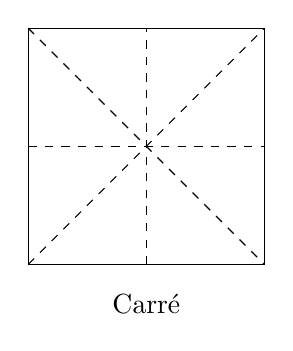
\begin{tikzpicture}[scale=0.5]
% Carré
\draw (0,0) rectangle (6,6);
\draw[dashed] (0,3) -- (6,3); % Axe de symétrie horizontal
\draw[dashed] (3,0) -- (3,6); % Axe de symétrie vertical
\draw[dashed] (0,6) -- (6,0); % Axe de symétrie diagonale haut-bas
\draw[dashed] (0,0) -- (6,6); % Axe de symétrie diagonale bas-haut
\node at (3,-1) {Carré};
\end{tikzpicture}
\hspace{1cm}
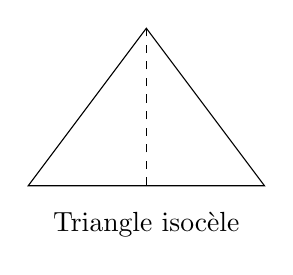
\begin{tikzpicture}[scale=0.5]
% Triangle isocèle
\draw (0,0) -- (6,0) -- (3,4) -- cycle;
\draw[dashed] (3,0) -- (3,4); % Axe de symétrie vertical
\node at (3,-1) {Triangle isocèle};
\end{tikzpicture}
\hspace{1cm}
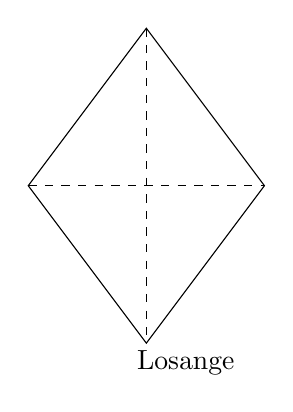
\begin{tikzpicture}[scale=0.5]
% Losange
\draw (0,0) -- (3,4) -- (6,0) -- (3,-4) -- cycle;
\draw[dashed] (3,4) -- (3,-4); % Axe de symétrie vertical
\draw[dashed] (0,0) -- (6,0); % Axe de symétrie horizontal
\node at (4,-4.5) {Losange};
\end{tikzpicture}

\vspace{1cm}

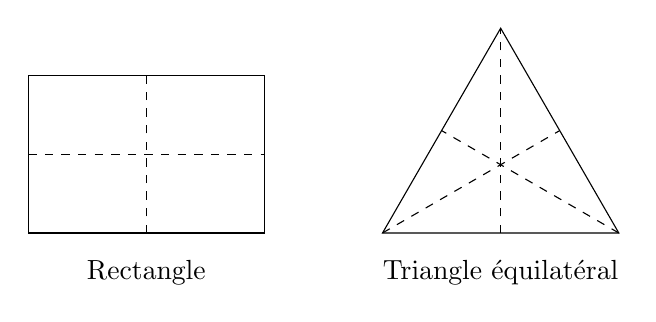
\begin{tikzpicture}[scale=0.5]
% Rectangle
\draw (-9,0) rectangle (-3,4);
\draw[dashed] (-6,0) -- (-6,4); % Axe de symétrie vertical
\draw[dashed] (-9,2) -- (-3,2); % Axe de symétrie horizontal
\node at (-6,-1) {Rectangle};

% Triangle équilatéral
\draw (0,0) -- (6,0) -- (3,5.2) -- cycle;
\draw[dashed] (3,0) -- (3,5.2); % Axe de symétrie vertical
\draw[dashed] (6,0) -- (1.5,2.6); % Axe de symétrie sommet droit
\draw[dashed] (0,0) -- (4.5,2.6); % Axe de symétrie sommet gauche
\node at (3,-1) {Triangle équilatéral};
\end{tikzpicture}
\hspace{1cm}
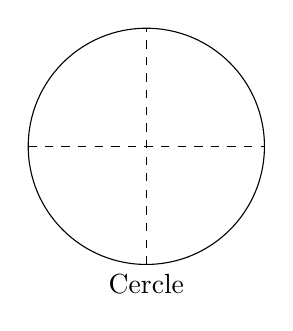
\begin{tikzpicture}[scale=0.5]
% Cercle
\draw (0,0) circle (3);
\draw[dashed] (-3,0) -- (3,0); % Axe de symétrie horizontal
\draw[dashed] (0,-3) -- (0,3); % Axe de symétrie vertical
\node at (0,-3.5) {Cercle};
\end{tikzpicture}
\end{center}
\end{PpT}

\end{pageCours}


\begin{pageAD} 
 

\Sf{Construire à l'aide du rapporteur, un angle de mesure donnée en degrés}
 
\ExoCad{Représenter.} 

 
 
\end{pageAD}


%%%%%%%%%%%%%%%%%%%%%%%%%%%%%%%%%%%%%%%%%%%%%%%%%%%%%%%%%%%%%%%%%%%
%%%%  Niveau 1
%%%%%%%%%%%%%%%%%%%%%%%%%%%%%%%%%%%%%%%%%%%%%%%%%%%%%%%%%%%%%%%%%%%
\begin{pageParcoursu} 

\ExoCu{Chercher. Communiquer.}

 
 
\end{pageParcoursu}


%%%%%%%%%%%%%%%%%%%%%%%%%%%%%%%%%%%%%%%%%%%%%%%%%%%%%%%%%%%%%%%%%%%
%%%%  Niveau 2
%%%%%%%%%%%%%%%%%%%%%%%%%%%%%%%%%%%%%%%%%%%%%%%%%%%%%%%%%%%%%%%%%%%
\begin{pageParcoursd} 


\ExoCd{Représenter. Calculer.} 

 
 
 
 
\end{pageParcoursd}

%%%%%%%%%%%%%%%%%%%%%%%%%%%%%%%%%%%%%%%%%%%%%%%%%%%%%%%%%%%%%%%%%%%
%%%%  Niveau 3
%%%%%%%%%%%%%%%%%%%%%%%%%%%%%%%%%%%%%%%%%%%%%%%%%%%%%%%%%%%%%%%%%%%
\begin{pageParcourst}


\ExoCt{Modéliser. Calculer.}

 
 
\end{pageParcourst}

%%%%%%%%%%%%%%%%%%%%%%%%%%%%%%%%%%%%%%%%%%%%%%%%%%%%%%%%%%%%%%%%%%%
%%%%  Brouillon
%%%%%%%%%%%%%%%%%%%%%%%%%%%%%%%%%%%%%%%%%%%%%%%%%%%%%%%%%%%%%%%%%%%


\begin{pageBrouillon} 
 
\ligne{32}



\end{pageBrouillon}



\begin{pageAuto} 

\ExoAuto
 
\ExoAuto
 



\ExoAuto

 

 



\end{pageAuto}



